%%%%%%%%%%%%%%%%%%%%%%%%%%%%%%%%%%%%%%%%%%%%%%%%%%%%%%%%%%%%%%%%%%%%%%%%%%%%%%%%
% Modelo LaTeX para o Projeto 1 de Introdução ao Reconhecimento de Padrões
% Disciplina: TI0097
% Professor: Dr. Guilherme de Alencar Barreto
%%%%%%%%%%%%%%%%%%%%%%%%%%%%%%%%%%%%%%%%%%%%%%%%%%%%%%%%%%%%%%%%%%%%%%%%%%%%%%%%

\documentclass[a4paper, 12pt]{article}

% --- PACOTES ESSENCIAIS ---
\usepackage[utf8]{inputenc} % Codificação de caracteres
\usepackage[T1]{fontenc}      % Codificação da fonte
\usepackage[portuguese]{babel} % Idioma do documento
\usepackage{geometry}         % Para ajustar as margens
\usepackage{amsmath}          % Para equações matemáticas
\usepackage{graphicx}         % Para incluir imagens
\usepackage{booktabs}         % Para tabelas com visual profissional
\usepackage{float}            % Para melhor controle de posicionamento de tabelas e figuras
\usepackage{hyperref}         % Para links (útil para referências)

% --- CONFIGURAÇÃO DAS MARGENS ---
\geometry{
    a4paper,
    total={170mm,257mm},
    left=20mm,
    top=20mm,
}

% --- INFORMAÇÕES DO CABEÇALHO ---
\title{
    \textbf{PROJETO 1: Reconhecimento de Faces} \\
    \large Disciplina: TI0097 - Introdução ao Reconhecimento de Padrões
}
\author{
    Gabriel Fruet \\
    \texttt{gabrielfruet@alu.ufc.br}
}
\date{\today}

% --- INÍCIO DO DOCUMENTO ---
\begin{document}

\maketitle % Cria o título com as informações acima

\begin{abstract}
    Este relatório apresenta os resultados obtidos no primeiro projeto da disciplina de Introdução ao Reconhecimento de Padrões. O objetivo do projeto é avaliar o desempenho de diferentes classificadores de padrões em um problema de reconhecimento de faces, utilizando a base de dados Yale A. As análises incluem a comparação de classificadores com e sem o uso da Análise de Componentes Principais (PCA) para pré-processamento e redução de dimensionalidade.
\end{abstract}

\section{Introdução}
O reconhecimento de faces é uma área de estudo proeminente em visão computacional e reconhecimento de padrões, com aplicações que vão desde sistemas de segurança e controle de acesso até a organização de fotos pessoais. Este projeto visa aplicar e comparar técnicas de classificação estudadas em sala de aula para resolver um problema prático de identificação de indivíduos a partir de imagens de suas faces.

% --- ATIVIDADES 1 E 2 ---
\section{Classificação Sem Aplicação de PCA}
Nesta seção, os classificadores foram treinados e testados utilizando os vetores de atributos extraídos diretamente das imagens redimensionadas, sem a aplicação da Análise de Componentes Principais (PCA). Foi utilizada uma proporção de 80\% dos dados para treinamento e 50 repetições independentes foram executadas para garantir a robustez estatística dos resultados.

\begin{table}[H]
    \centering
    \caption{Resultados de desempenho dos classificadores sem PCA.}
    \label{tab:sem_pca}
    \begin{tabular}{lcccccc}
        \toprule
        \textbf{Classificador} & \textbf{Média} & \textbf{Mínimo} & \textbf{Máximo} & \textbf{Mediana} & \textbf{Desvio Padrão} & \textbf{Tempo total (s)} \\
        \midrule

        Quadrático         & 5.6970   & 0.0000   & 15.1515  & 6.0606   & 3.6685         & 252.2501\\
        Variante 1         & 80.7879  & 66.6667  & 93.9394  & 80.3030  & 5.5417         & 127.3319\\
        Variante 2         & 3.3939   & 0.0000   & 15.1515  & 3.0303   & 3.9575         & 131.7177\\
        Variante 3         & 3.0303   & 0.0000   & 9.0909   & 3.0303   & 2.9691         & 136.7711\\
        Variante 4         & 17.3333  & 3.0303   & 27.2727  & 18.1818  & 6.9112         & 215.7832\\
        DMC                & 77.3333  & 63.6364  & 87.8788  & 78.7879  & 5.8522         & 0.1118\\
        1NN                & 79.7576  & 63.6364  & 90.9091  & 81.8182  & 6.1937         & 0.6537\\
        Máxima Correlação  & 77.2727  & 54.5455  & 87.8788  & 78.7879  & 6.3057         & 0.0171\\
        \bottomrule
    \end{tabular}
\end{table}

\subsection*{Análise dos Resultados (Questões 1, 2 e 3)}
\paragraph{Questão 1:} O que se pode concluir sobre os desempenhos dos classificadores avaliados?

Os classificadores baseados em distância euclidiana como DMC, 1-NN e MaxCorr
tiveram uma performance muito boa e um \textit{runtime} extremamento baixo quando comparado com os baseados
em distância de mahalanobis.
Para compararmos, o runtime do MaxCorr foi mais de 10 mil vezes mais rapido que
o Quadrático.

\paragraph{Questão 2:} Qual deles teve o melhor desempenho em relação à taxa de acerto? E em relação ao tempo?

Em relação a taxa de acerto, o que teve melhores resultados foi a Variante 1
(Thikonov) do Quadrático. Um classificador que se aproximou bastante foi o
1-NN, que teve uma taxa de acerto levemente pior e um desvio padrão levemente
pior também. Vale ressaltar que apesar de pequena diferença, o 1-NN foi 200
vezes mais rápido que a Variante 1.

Sobre tempo de execução, a variante de MaxCorr foi a mais rápida, sendo 2 vezes mais rápida que
a segunda mais rápida e mais de 10 mil vezes mais rápida que a mais lenta. Apesar da velocidade,
sua performance foi muito boa quando comparado com os classificadores baseados em distância de Mahalanobis.





\paragraph{Questão 3:} Houve problemas de inversão das matrizes de covariância? Se sim, para quais classificadores? Este problema foi contornado por alguma das variantes avaliadas? Se sim, descreva sucintamente o mecanismo usado para resolvê-lo.
% Escreva sua resposta aqui.

Sim, houveram problemas na inversão da matriz de covariância especialmente para o Quadrático,
por isso o runtime dele foi tão mais alto que as outras variantes. Já que, a heurística que usei para
inversão foi a seguinte: \texttt{Tenta inverter, se falhar, use a pseudo-inversa}. Apesar dos outros não
terem problemas de erro na inversão da matriz de covariância, todos tiveram um posto extremamente baixo,
exceto a Variante 1, que aplicou regularização de Thikonov, que diminui a colinearidade das features..




\section{Classificação com PCA (Sem Redução de Dimensionalidade)}
Aqui, o PCA foi aplicado aos dados com o objetivo de descorrelacionar os atributos, mas mantendo a dimensionalidade original. O processo de treino e teste foi repetido nas mesmas condições da seção anterior.

\begin{table}[H]
    \centering
    \caption{Resultados com aplicação de PCA sem redução de dimensionalidade(q=900).}
    \label{tab:pca_sem_reducao}
    \begin{tabular}{lcccccc}
        \toprule
        \textbf{Classificador} & \textbf{Média} & \textbf{Mínimo} & \textbf{Máximo} & \textbf{Mediana} & \textbf{Desvio Padrão} & \textbf{Tempo (s)} \\
        \midrule
        Quadrático         & 6.4848   & 0.0000   & 18.1818  & 6.0606   & 4.2429         & 230.1835\\
        Variante 1         & 81.0909  & 63.6364  & 93.9394  & 81.8182  & 6.2268         & 123.0351\\
        Variante 2         & 6.9091   & 0.0000   & 15.1515  & 6.0606   & 3.7380         & 234.7739\\
        Variante 3         & 6.8485   & 0.0000   & 15.1515  & 6.0606   & 3.9654         & 233.9609\\
        Variante 4         & 6.1818   & 0.0000   & 12.1212  & 6.0606   & 3.0279         & 610.1199\\
        DMC                & 78.7273  & 63.6364  & 93.9394  & 78.7879  & 6.7349         & 0.0362\\
        1NN                & 77.9394  & 66.6667  & 96.9697  & 78.7879  & 6.2703         & 0.4945\\
        Máxima Correlação  & 78.5455  & 63.6364  & 93.9394  & 78.7879  & 6.3806         & 0.0161\\
        \bottomrule
    \end{tabular}
\end{table}

\subsection*{Análise dos Resultados (Questão 4)}
\paragraph{Questão 4:} (i) O que se pode concluir sobre os desempenhos dos classificadores avaliados? Houve alguma mudança (melhora ou piora) nos desempenhos em relação à tabela anterior? (ii) Note que, com a aplicação de PCA, a matriz de covariância dos dados transformados é diagonal. Isso faz com que o classificador quadrático e a Variante 4 sejam teoricamente equivalentes. Estes classificadores tiveram de fato desempenho equivalente?

\begin{itemize}
    \item[(i)] Houve uma melhora significativa para as variantes 2 e 3 do quadrático, com uma média de acerto
        sendo quase o dobro comparando sem aplicar o PCA. A variante 4 teve uma grande piora, tendo uma performance
        4x menor que na sua contraparte sem aplicar o PCA.
    \item[(ii)] Não tiveram resultados parecidos, contrariando a teória. A variante 4 ainda teve uma taxa de acerto
        3x maior que sua versão sem PCA. 
        Fui analisar o porquê disso e, apesar da aplicação do PCA, por não reduzirmos o número de componentes,
        algumas componentes ficam "zeradas", trazendo um grande ruído pra matriz de covariância. Já que o número
        de componentes principais vai ser o mínimo entre o número de amostras e o número de features.
\end{itemize}

% Escreva sua resposta aqui.

\section{Classificação com PCA (Com Redução de Dimensionalidade)}
Nesta etapa, o PCA foi utilizado para reduzir a dimensionalidade do espaço de atributos, preservando 98\% da variância total dos dados originais.

\subsection*{Análise dos Resultados (Questões 5 e 6)}
\paragraph{Questão 5:} Qual foi a dimensão de redução $q$ escolhida, de modo a preservar 98\% da informação do conjunto de dados original?
% Escreva sua resposta aqui.

\begin{table}[H]
    \centering
    \caption{Resultados com aplicação de PCA com redução de dimensionalidade ($q = \text{seu valor}$).}
    \label{tab:pca_com_reducao}
    \begin{tabular}{lcccccc}
        \toprule
        \textbf{Classificador} & \textbf{Média} & \textbf{Mínimo} & \textbf{Máximo} & \textbf{Mediana} & \textbf{Desvio Padrão} & \textbf{Tempo (s)} \\
        \midrule
        Quadrático         & 2.8485   & 0.0000   & 12.1212   & 3.0303   & 2.8690         & 0.3910\\
        Variante 1         & 81.5758  & 63.6364  & 90.9091   & 81.8182  & 5.4153         & 0.3654\\
        Variante 2         & 95.9394  & 84.8485  & 100.0000  & 96.9697  & 3.3531         & 0.3794\\
        Variante 3         & 92.2424  & 81.8182  & 100.0000  & 93.9394  & 4.7008         & 0.3812\\
        Variante 4         & 73.8182  & 63.6364  & 87.8788   & 74.2424  & 6.0836         & 0.3152\\
        DMC                & 78.3636  & 60.6061  & 90.9091   & 78.7879  & 7.5456         & 0.0093\\
        1NN                & 80.0606  & 66.6667  & 93.9394   & 78.7879  & 6.7513         & 0.0134\\
        Máxima Correlação  & 76.5455  & 63.6364  & 90.9091   & 75.7576  & 7.0368         & 0.0082\\
        \bottomrule
    \end{tabular}
\end{table}

\begin{figure}
    \centering
    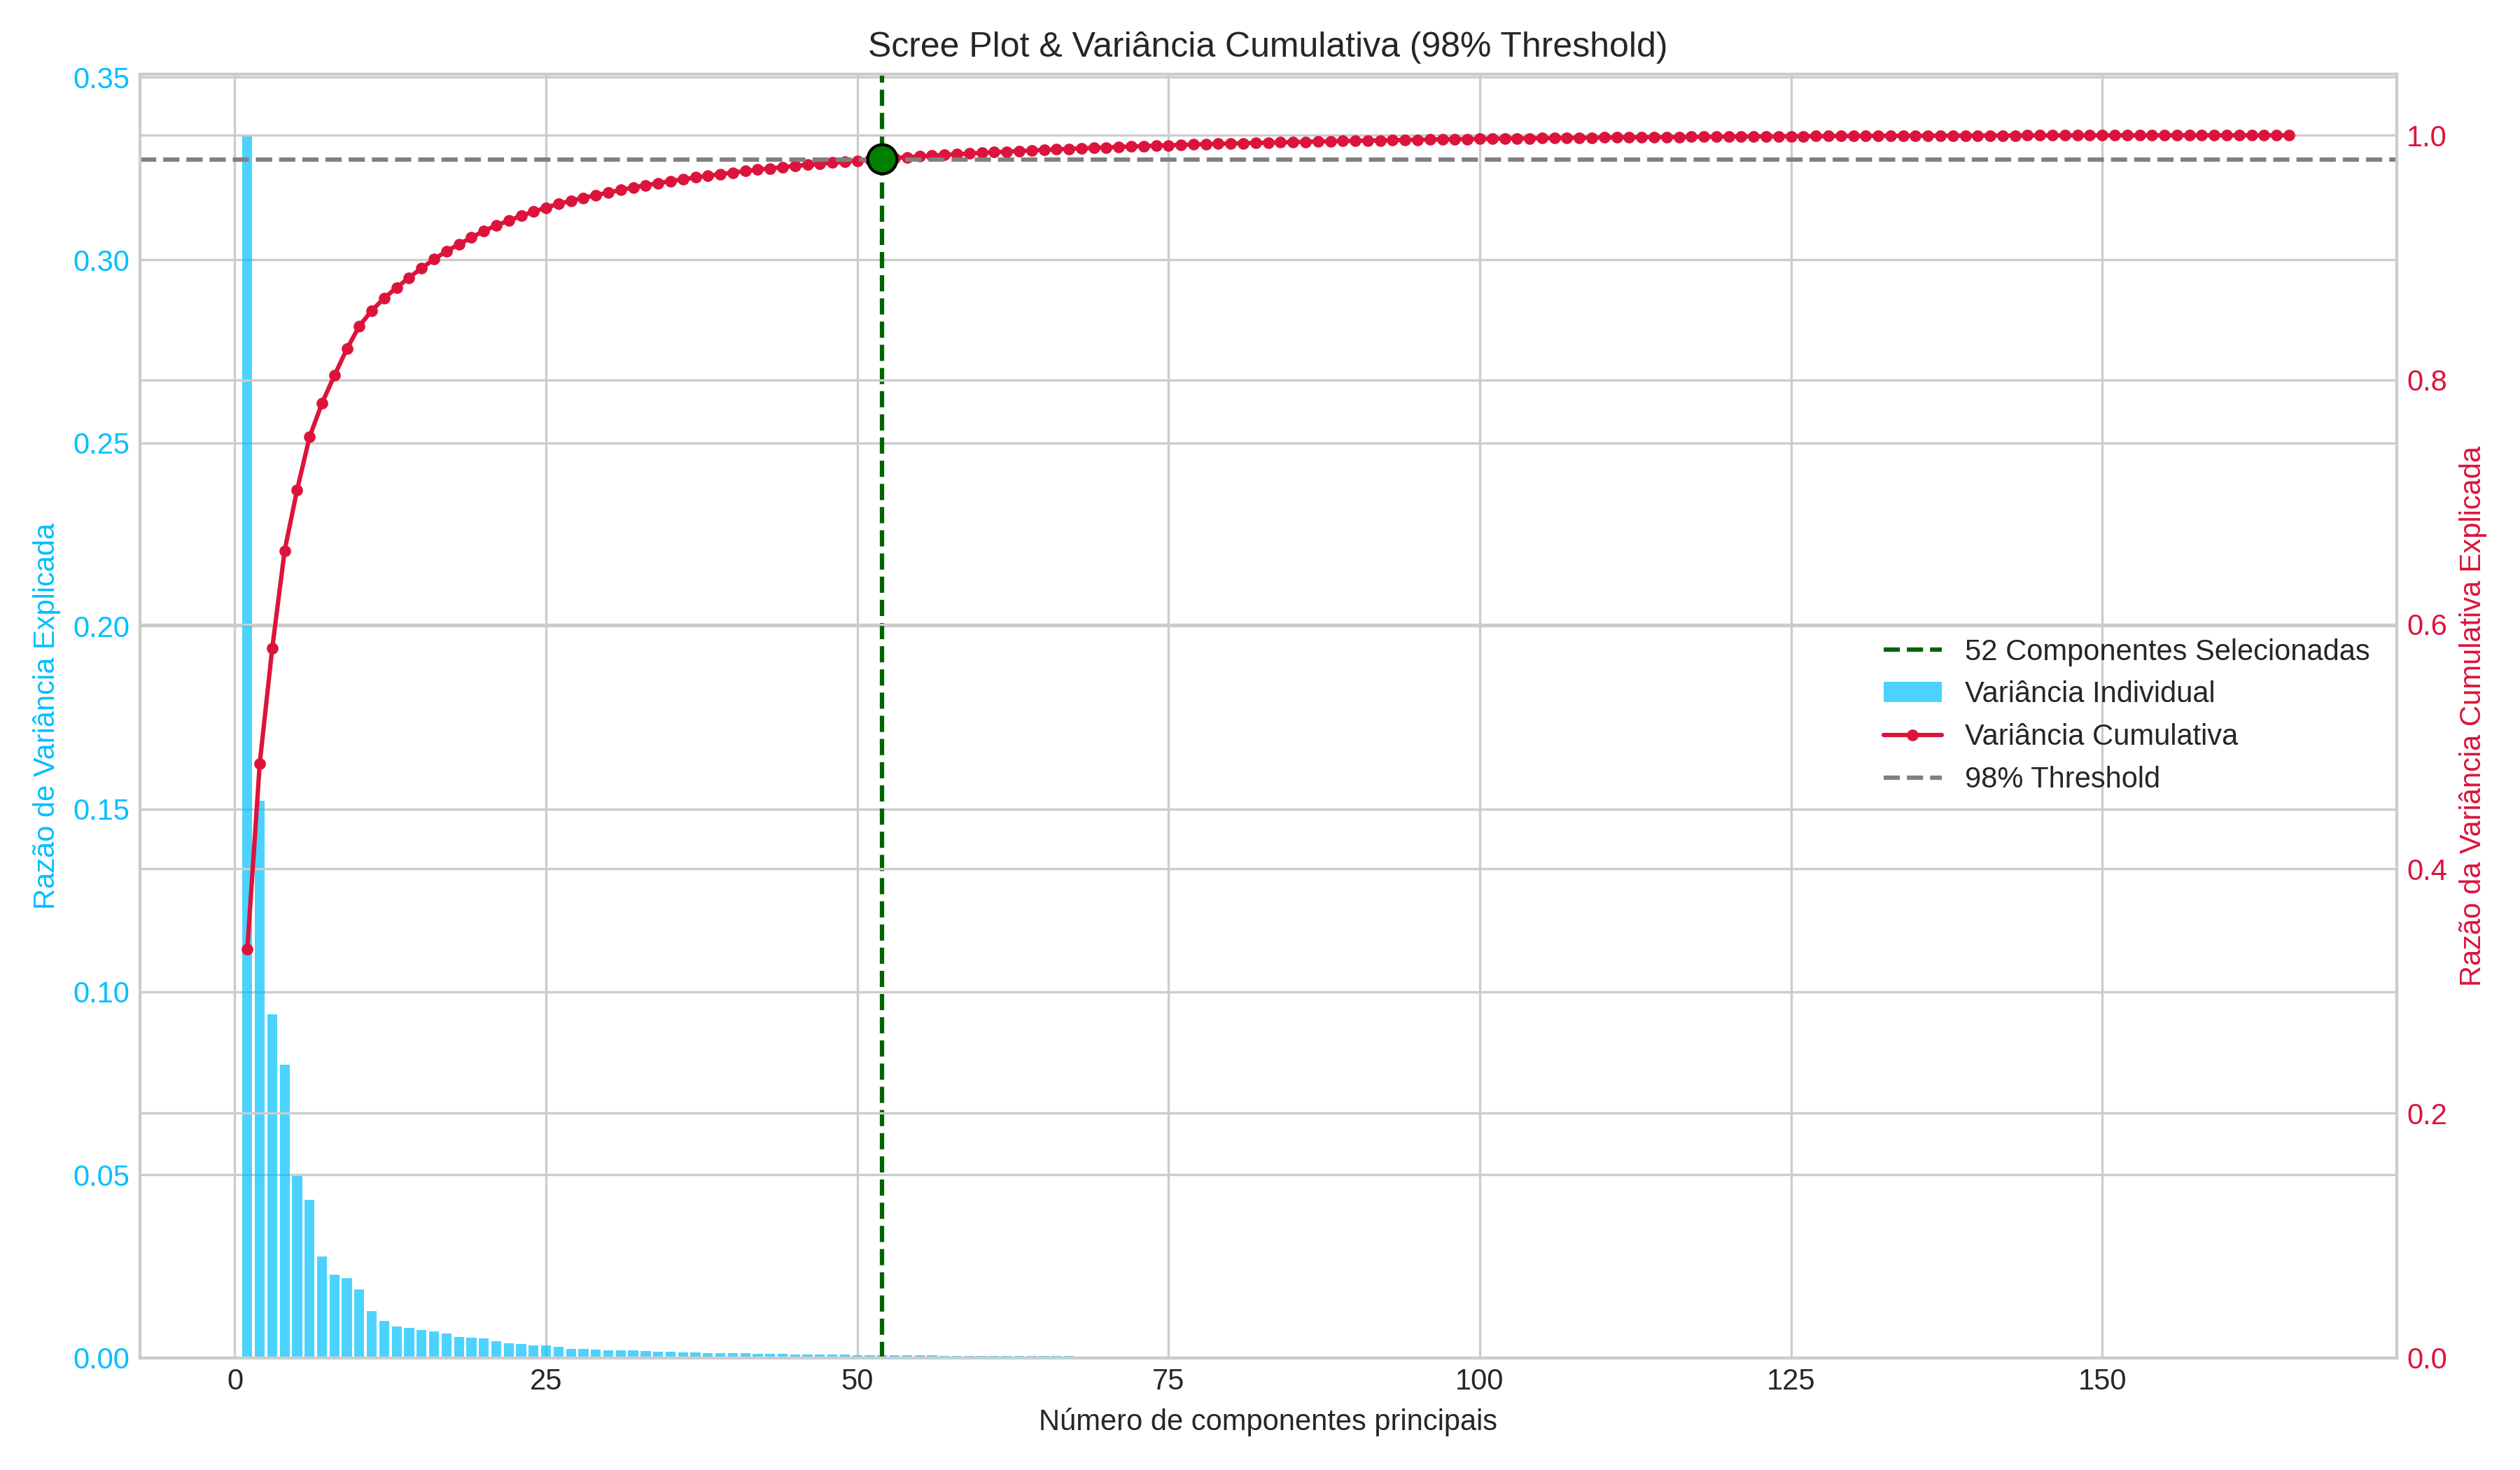
\includegraphics[width=0.7\textwidth]{./recfaces_30_pca_98_scree_plot.png}
    \caption{Scree plot para variância explicada 98\%}
\end{figure}

\paragraph{Questão 6:} O que se pode concluir sobre os desempenhos dos classificadores com a redução de dimensionalidade via PCA? Houve alguma mudança (melhora ou piora) em relação à tabela anterior? Quais classificadores pioraram/melhoraram?
% Escreva sua resposta aqui.
Todos os classificadores melhoraram, exceto o quadrático. Vale destacar que o runtime diminuiu em aproximadamente
em 50 vezes para os classificadores baseados em QDA.

Os classificadores que mais melhoraram foram as variantes 1 (Thikonov), 2 (Pooled), 3 (Friedman), 4 (Diagonal).

Os classificadores baseados em distância euclidiana não variaram muito em
nenhumas das três técnicas aplicadas até agora(sem PCA, com PCA e com PCA com redução de dimensionalidade)


\section{Análise com Transformação Box-Cox e PCA}
\subsection*{Análise dos Resultados (Questão 7)}


\begin{table}[H]
    \centering
    \caption{Resultados com aplicação de PCA com redução de dimensionalidade ($q = \text{seu valor}$).}
    \label{tab:pca_com_reducao}
    \begin{tabular}{lcccccc}
        \toprule
        \textbf{Classificador} & \textbf{Média} & \textbf{Mínimo} & \textbf{Máximo} & \textbf{Mediana} & \textbf{Desvio Padrão} & \textbf{Tempo (s)} \\
        \midrule
        Quadrático         & 2.3636   & 0.0000   & 12.1212   & 3.0303   & 2.8614         & 0.4016\\
        Variante 1         & 89.0909  & 75.7576  & 96.9697   & 87.8788  & 4.1989         & 0.3749\\
        Variante 2         & 97.6364  & 90.9091  & 100.0000  & 96.9697  & 2.5201         & 0.3840\\
        Variante 3         & 96.6667  & 87.8788  & 100.0000  & 96.9697  & 3.2213         & 0.3911\\
        Variante 4         & 69.0303  & 54.5455  & 84.8485   & 69.6970  & 7.6970         & 0.3338\\
        DMC                & 86.1818  & 75.7576  & 96.9697   & 86.3636  & 5.7547         & 0.0096\\
        1NN                & 88.1818  & 69.6970  & 96.9697   & 87.8788  & 6.1881         & 0.0140\\
        Máxima Correlação  & 84.4848  & 69.6970  & 96.9697   & 84.8485  & 5.9270         & 0.0082\\
        \bottomrule
    \end{tabular}
\end{table}
% Preencha a tabela de resultados aqui se desejar, ou apenas discuta os resultados.
\paragraph{Questão 7:} Houve alguma mudança (melhora ou piora) nos desempenhos dos classificadores em relação aos resultados da Atividade 6? Quais classificadores pioraram/melhoraram de desempenho com a aplicação da transformação BOX-COX juntamente com PCA?


Todos os classificadores melhoraram, em especial a variante 2, que tomou o pódio. O único que perfomou pior
foi o quadrático, que teve sua melhor performance usando PCA sem redução de dimensionalidade.


\section{Controle de Acesso}
\subsection*{Análise dos Resultados (Questão 8)}
% Preencha a tabela de resultados aqui.
\paragraph{Questão 8:} Calcule os seguintes índices de desempenho para os classificadores implementados: acurácia, taxa de falsos negativos e taxa de falsos positivos, sensibilidade e precisão. Os valores devem ser médios com inclusão de medida de dispersão (e.g., desvio padrão) para 50 rodadas.
% Escreva sua resposta aqui.

\section{Conclusão}
% Escreva aqui uma conclusão geral sobre o projeto, resumindo os principais achados,
% as dificuldades encontradas e o aprendizado obtido.

\end{document}

